\documentclass[12pt, a4paper]{article}

\usepackage[utf8]{inputenc}
\usepackage[T1]{fontenc}
\usepackage{amsmath, amssymb, amsthm}
\usepackage{algorithm}
\usepackage{algpseudocode}
\usepackage{graphicx}
\usepackage{subcaption}
\usepackage{booktabs}
\usepackage{hyperref}
\usepackage{geometry}
\usepackage{float}
\usepackage{multirow}
\usepackage{xcolor}
\usepackage{cite}
\usepackage{lmodern}

\geometry{margin=2.5cm}

\hypersetup{
    colorlinks=true,
    linkcolor=blue,
    urlcolor=blue,
    citecolor=blue
}

\title{%
    \textbf{Enhancing GPS Accuracy with Machine Learning} \\[0.5em]
    \large A Comparative Analysis of Algorithms
}
\author{Urban Fleet Management System (UFMS) Research}
\date{Ho Chi Minh City, 2025}

\begin{document}

\maketitle
\tableofcontents
\newpage

% ─────────────────────────────────────────────────────────────────────────────
\section{Introduction}
% ─────────────────────────────────────────────────────────────────────────────

Global Navigation Satellite System (GNSS) receivers mounted on urban buses
continuously emit positional fixes at regular intervals. In dense urban
environments such as Ho Chi Minh City, these raw GPS observations are corrupted
by multipath reflections, atmospheric delays, and receiver clock drift,
producing positional errors that typically range from 5 to 30 metres under
favourable conditions and may exceed 100 metres in deep urban canyons.

The downstream consequences of unfiltered GPS noise are significant: fleet
management dashboards display erratic vehicle traces, estimated time-of-arrival
(ETA) computations are destabilised, and anomaly-detection algorithms
misclassify legitimate stops as off-route events. An effective noise-reduction
pipeline is therefore a prerequisite for reliable fleet intelligence.

This report describes and evaluates multiple approaches to GPS trajectory
smoothing applied to a full operational day of bus GPS data collected on
18 March 2025 across nine routes in Ho Chi Minh City, comprising 720,088
positional fixes from 123 vehicles. Each algorithm is presented as a
self-contained section (Section~\ref{sec:algorithms}) and evaluated against
the shared metrics defined in Section~\ref{sec:metrics}. Comparative results
are reported in Section~\ref{sec:results}.

% ─────────────────────────────────────────────────────────────────────────────
\section{Dataset}
\label{sec:dataset}
% ─────────────────────────────────────────────────────────────────────────────

All algorithms in this report are evaluated on the same dataset, summarised
in Table~\ref{tab:dataset}.

\begin{table}[H]
\centering
\caption{Dataset statistics}
\label{tab:dataset}
\begin{tabular}{lrr}
\toprule
\textbf{Property} & \textbf{Value} \\
\midrule
Date of collection       & 18 March 2025 \\
Routes                   & 9 (nos.\ 29, 41, 57, 61, 84, 99, 102, 141, 151) \\
Vehicles                 & 123 \\
Total GPS pings          & 720,088 \\
Average pings/vehicle    & 5,854 \\
GPS speed availability   & $\approx$50\% (remainder computed via haversine) \\
Average \% pings at stop & 26.5\% \\
Route geometry source    & OpenStreetMap (\texttt{hcmc\_bus\_routes.gpkg}) \\
Timetable source         & Operational GTFS (\texttt{stop\_times.csv}) \\
\bottomrule
\end{tabular}
\end{table}

% ─────────────────────────────────────────────────────────────────────────────
\section{Evaluation Metrics}
\label{sec:metrics}
% ─────────────────────────────────────────────────────────────────────────────

Two complementary metrics are employed across all algorithms.

\paragraph{Mean Distance to Route (MDR).}
For a filtered trajectory $\{\tilde{\mathbf{p}}_k\}_{k=1}^{N}$, MDR quantifies
average spatial deviation from the nominal route polyline $\mathcal{R}$:

\begin{equation}
    \text{MDR} = \frac{1}{N}\sum_{k=1}^{N}
        d\!\left(\tilde{\mathbf{p}}_k,\, \mathcal{R}\right) \cdot D_{\text{deg}}
    \quad [\text{metres}]
    \label{eq:mdr}
\end{equation}

Lower MDR indicates tighter adherence to the expected route path.

\paragraph{Mean Heading Change (MHC).}
MHC quantifies trajectory smoothness by measuring the average absolute change
in instantaneous bearing between consecutive pings:

\begin{equation}
    \text{MHC} = \frac{1}{N-2}
        \sum_{k=2}^{N-1} \left|\,\theta_k - \theta_{k-1}\,\right|
    \quad [{}^\circ]
    \label{eq:mhc}
\end{equation}

\noindent where $\theta_k = \arctan2(\Delta\lambda_k,\,\Delta\phi_k)$ is the
bearing from ping $k-1$ to ping $k$. Lower MHC indicates a smoother,
less jittery trajectory.

\paragraph{Improvement percentage.}
For any metric $M$, the improvement of a filtered trajectory relative to raw
GPS is reported as:

\begin{equation}
    \Delta M [\%] = \frac{M_{\text{raw}} - M_{\text{filtered}}}{M_{\text{raw}}} \times 100
    \label{eq:impr_pct}
\end{equation}

A positive value indicates improvement; a negative value indicates
deterioration.

% ─────────────────────────────────────────────────────────────────────────────
\section{Algorithms}
\label{sec:algorithms}
% ─────────────────────────────────────────────────────────────────────────────

Each subsection below describes one algorithm: its theoretical background,
implementation, and per-algorithm notes. Aggregate comparison across all
algorithms is deferred to Section~\ref{sec:results}.

% ─────────────────────────────────────────────────────────────────────────────
\subsection{Standard Kalman Filter (KF)}
\label{sec:kf}
% ─────────────────────────────────────────────────────────────────────────────

\subsubsection{State-Space Formulation}

The Kalman filter \cite{kalman1960} operates on a linear discrete-time
dynamical system defined by the state-transition and observation equations:

\begin{align}
    \mathbf{x}_k &= \mathbf{F}\,\mathbf{x}_{k-1} + \mathbf{w}_{k-1},
    \quad \mathbf{w}_{k-1} \sim \mathcal{N}(\mathbf{0},\, \mathbf{Q})
    \label{eq:state_transition} \\
    \mathbf{z}_k &= \mathbf{H}\,\mathbf{x}_k + \mathbf{v}_k,
    \quad \mathbf{v}_k \sim \mathcal{N}(\mathbf{0},\, \mathbf{R})
    \label{eq:observation}
\end{align}

\noindent where $\mathbf{x}_k \in \mathbb{R}^n$ is the latent state vector at
time step $k$, $\mathbf{z}_k \in \mathbb{R}^m$ is the observation vector,
$\mathbf{F}$ is the state-transition matrix, $\mathbf{H}$ is the observation
matrix, $\mathbf{Q}$ is the process-noise covariance, and $\mathbf{R}$ is the
measurement-noise covariance. Both noise terms are assumed to be zero-mean
white Gaussian and mutually uncorrelated.

\subsubsection{State Vector for GPS Tracking}

For bus GPS tracking, the state vector encodes both position and velocity in
geodetic coordinates:

\begin{equation}
    \mathbf{x}_k =
    \begin{bmatrix}
        \phi_k \\ \lambda_k \\ \dot{\phi}_k \\ \dot{\lambda}_k
    \end{bmatrix}
    \label{eq:state_vector}
\end{equation}

\noindent where $\phi_k$ is latitude, $\lambda_k$ is longitude, and
$\dot{\phi}_k,\,\dot{\lambda}_k$ are their respective rates of change. At
city scale the curvature of the geoid is negligible, so Equations
\eqref{eq:state_transition}--\eqref{eq:observation} remain linear in
$(\phi, \lambda)$.

The state-transition matrix embeds a constant-velocity (CV) kinematic model
with unit time step $\Delta t = 1$:

\begin{equation}
    \mathbf{F} =
    \begin{bmatrix}
        1 & 0 & \Delta t & 0 \\
        0 & 1 & 0 & \Delta t \\
        0 & 0 & 1 & 0 \\
        0 & 0 & 0 & 1
    \end{bmatrix},
    \qquad
    \mathbf{H} =
    \begin{bmatrix}
        1 & 0 & 0 & 0 \\
        0 & 1 & 0 & 0
    \end{bmatrix}
    \label{eq:matrices}
\end{equation}

GPS receivers observe only position, hence $\mathbf{H}$ projects the full
state to the two-dimensional observation space.

\subsubsection{Recursive Estimation Equations}

The Kalman filter alternates between a \emph{predict} step, which propagates
the state estimate forward in time using the motion model, and an \emph{update}
step, which corrects the prediction using the incoming measurement.

\paragraph{Predict Step}

\begin{align}
    \hat{\mathbf{x}}^-_k &= \mathbf{F}\,\hat{\mathbf{x}}_{k-1}
    \label{eq:predict_state} \\
    \mathbf{P}^-_k &= \mathbf{F}\,\mathbf{P}_{k-1}\,\mathbf{F}^\top + \mathbf{Q}
    \label{eq:predict_cov}
\end{align}

\noindent where $\hat{\mathbf{x}}^-_k$ is the \emph{a priori} state estimate
and $\mathbf{P}^-_k$ is its associated covariance matrix.

\paragraph{Update Step}

\begin{align}
    \boldsymbol{\nu}_k &= \mathbf{z}_k - \mathbf{H}\,\hat{\mathbf{x}}^-_k
    \label{eq:innovation} \\
    \mathbf{S}_k &= \mathbf{H}\,\mathbf{P}^-_k\,\mathbf{H}^\top + \mathbf{R}
    \label{eq:innovation_cov} \\
    \mathbf{K}_k &= \mathbf{P}^-_k\,\mathbf{H}^\top\,\mathbf{S}_k^{-1}
    \label{eq:kalman_gain} \\
    \hat{\mathbf{x}}_k &= \hat{\mathbf{x}}^-_k + \mathbf{K}_k\,\boldsymbol{\nu}_k
    \label{eq:update_state} \\
    \mathbf{P}_k &= \left(\mathbf{I} - \mathbf{K}_k\,\mathbf{H}\right)\mathbf{P}^-_k
    \label{eq:update_cov}
\end{align}

\noindent The vector $\boldsymbol{\nu}_k$ is the \emph{innovation} (residual
between measurement and prediction), $\mathbf{S}_k$ is the innovation
covariance, and $\mathbf{K}_k$ is the \emph{Kalman gain}, which determines
the weight assigned to the new measurement relative to the prior prediction.

\subsubsection{Pseudocode}

\begin{algorithm}[H]
\caption{Standard Kalman Filter for GPS Tracking}
\label{alg:standard_kf}
\begin{algorithmic}[1]
\State \textbf{Initialise:} $\hat{\mathbf{x}}_0 \leftarrow [\phi_0,\,\lambda_0,\,0,\,0]^\top$,\;
       $\mathbf{P}_0 \leftarrow \mathbf{I}_4$
\For{each GPS ping $(\phi_k,\,\lambda_k,\,t_k)$ in time order}
    \State \Comment{\textit{Predict}}
    \State $\hat{\mathbf{x}}^-_k \leftarrow \mathbf{F}\,\hat{\mathbf{x}}_{k-1}$
    \State $\mathbf{P}^-_k \leftarrow \mathbf{F}\,\mathbf{P}_{k-1}\,\mathbf{F}^\top + \mathbf{Q}$
    \State \Comment{\textit{Update}}
    \State $\mathbf{z}_k \leftarrow [\phi_k,\,\lambda_k]^\top$
    \State $\boldsymbol{\nu}_k \leftarrow \mathbf{z}_k - \mathbf{H}\,\hat{\mathbf{x}}^-_k$
    \State $\mathbf{S}_k \leftarrow \mathbf{H}\,\mathbf{P}^-_k\,\mathbf{H}^\top + \mathbf{R}$
    \State $\mathbf{K}_k \leftarrow \mathbf{P}^-_k\,\mathbf{H}^\top\,\mathbf{S}_k^{-1}$
    \State $\hat{\mathbf{x}}_k \leftarrow \hat{\mathbf{x}}^-_k + \mathbf{K}_k\,\boldsymbol{\nu}_k$
    \State $\mathbf{P}_k \leftarrow (\mathbf{I} - \mathbf{K}_k\,\mathbf{H})\,\mathbf{P}^-_k$
    \State \textbf{output} $\hat{\mathbf{x}}_k[0:2]$ \Comment{filtered $(\phi, \lambda)$}
\EndFor
\end{algorithmic}
\end{algorithm}

\subsubsection{Limitations in Urban Bus Applications}

While the standard KF is theoretically optimal under its Gaussian assumptions,
three structural limitations reduce its effectiveness for urban bus tracking:

\begin{enumerate}
    \item \textbf{Route ignorance.} The CV model has no knowledge of the fixed
          route geometry. Filtered positions may drift perpendicular to the road
          by tens of metres, particularly during turns where the lag of the CV
          model is most pronounced.

    \item \textbf{Stop blindness.} Buses dwell at scheduled stops for periods
          ranging from 15 to 120 seconds. A constant-velocity model incorrectly
          continues to propagate velocity through these stationary intervals,
          accumulating positional error.

    \item \textbf{Static noise parameters.} The process-noise covariance
          $\mathbf{Q}$ is held constant, whereas the true dynamical uncertainty
          varies dramatically between cruising (high $\mathbf{Q}$) and stopped
          (low $\mathbf{Q}$) states.
\end{enumerate}

% ─────────────────────────────────────────────────────────────────────────────
\subsection{Map-Matched Kalman Filter with Scheduled Stop Detection (MM-KF)}
\label{sec:mmkf}
% ─────────────────────────────────────────────────────────────────────────────

\subsubsection{Core Idea}

The MM-KF addresses the three limitations of the standard KF
(Section~\ref{sec:kf}) by augmenting the standard KF pipeline with two
domain-knowledge components:

\begin{enumerate}
    \item \textbf{Scheduled stop detection.} The GTFS \texttt{stop\_times}
          table provides, for each vehicle–trip pair, the scheduled arrival
          time $t^{\text{arr}}_s$, dwell time $d_s$, and departure time
          $t^{\text{dep}}_s$ at every stop $s$. A ping at time $t_k$ is
          classified as \emph{at-stop} if
          \[
              \exists\, s : t^{\text{arr}}_s \leq t_k \leq t^{\text{dep}}_s
          \]
          This binary classification gates between two process-noise regimes.

    \item \textbf{Geometric map-matching.} After each KF update, the filtered
          position is projected onto the nearest point of the known route
          polyline $\mathcal{R}$ — provided it lies within a configurable snap
          threshold $d_{\max}$. This enforces the physical constraint that a
          bus must travel along its designated route.
\end{enumerate}

\subsubsection{Adaptive Process Noise}

Let $\mathcal{S}(t_k)$ be the indicator function that equals 1 if ping $k$
falls within a scheduled stop window and 0 otherwise. The process-noise matrix
is selected adaptively:

\begin{equation}
    \mathbf{Q}_k =
    \begin{cases}
        \mathbf{Q}_{\text{stopped}} & \text{if } \mathcal{S}(t_k) = 1 \\
        \mathbf{Q}_{\text{moving}}  & \text{otherwise}
    \end{cases}
    \label{eq:adaptive_Q}
\end{equation}

The two regimes are parameterised as diagonal matrices:

\begin{align}
    \mathbf{Q}_{\text{moving}}  &= \operatorname{diag}
        \!\left(10^{-8},\; 10^{-8},\; 10^{-6},\; 10^{-6}\right)
    \label{eq:Q_moving} \\
    \mathbf{Q}_{\text{stopped}} &= \operatorname{diag}
        \!\left(10^{-10},\; 10^{-10},\; 10^{-3},\; 10^{-3}\right)
    \label{eq:Q_stopped}
\end{align}

In $\mathbf{Q}_{\text{stopped}}$, the positional diagonal entries are three
orders of magnitude smaller than in $\mathbf{Q}_{\text{moving}}$, strongly
anchoring the position estimate. Conversely, the velocity diagonal entries are
large, allowing the model to rapidly decay stored velocity to zero without
constraining subsequent acceleration when the bus departs.

\subsubsection{Map-Matching Projection}

Let $\hat{\mathbf{p}}_k = [\hat{\phi}_k,\,\hat{\lambda}_k]^\top$ denote the
KF-updated position. The map-matching operator
$\Pi_{\mathcal{R}} : \mathbb{R}^2 \to \mathcal{R}$ projects this point onto
the route polyline:

\begin{equation}
    \tilde{\mathbf{p}}_k =
    \begin{cases}
        \Pi_{\mathcal{R}}(\hat{\mathbf{p}}_k)
            & \text{if } d\!\left(\hat{\mathbf{p}}_k,\, \mathcal{R}\right)
              \cdot D_{\text{deg}} \leq d_{\max} \\
        \hat{\mathbf{p}}_k & \text{otherwise}
    \end{cases}
    \label{eq:map_match}
\end{equation}

\noindent where $d(\cdot,\mathcal{R})$ is the Euclidean distance in degrees to
the nearest point on $\mathcal{R}$, $D_{\text{deg}} = 111{,}000\,\text{m/deg}$
is the degree-to-metre conversion factor, and $d_{\max} = 150\,\text{m}$ is
the snap threshold. The threshold prevents erroneous snapping of outlier pings
(e.g., during depot ingress or GPS signal loss) to a distant portion of the
route.

The projection $\Pi_{\mathcal{R}}$ is computed as the nearest point on the
union geometry of all direction polylines of route $\mathcal{R}$ using the
Shapely computational geometry library.

\subsubsection{Full Algorithm}

\begin{algorithm}[H]
\caption{Map-Matched Kalman Filter with Scheduled Stop Detection (MM-KF)}
\label{alg:mm_kf}
\begin{algorithmic}[1]
\Require Route polyline $\mathcal{R}$, GTFS stop schedule
         $\{(t^{\text{arr}}_s, t^{\text{dep}}_s)\}$,
         snap threshold $d_{\max}$
\State \textbf{Initialise:} $\hat{\mathbf{x}}_0 \leftarrow
       [\phi_0,\,\lambda_0,\,0,\,0]^\top$,\;
       $\mathbf{P}_0 \leftarrow \mathbf{I}_4$
\For{each GPS ping $(\phi_k,\,\lambda_k,\,t_k)$ in datetime order}
    \State \Comment{\textit{Step 1 — Stop detection}}
    \If{$\exists\,s : t^{\text{arr}}_s \leq t_k \leq t^{\text{dep}}_s$}
        \State $\mathbf{Q}_k \leftarrow \mathbf{Q}_{\text{stopped}}$
    \Else
        \State $\mathbf{Q}_k \leftarrow \mathbf{Q}_{\text{moving}}$
    \EndIf
    \State \Comment{\textit{Step 2 — Kalman predict}}
    \State $\hat{\mathbf{x}}^-_k \leftarrow \mathbf{F}\,\hat{\mathbf{x}}_{k-1}$
    \State $\mathbf{P}^-_k \leftarrow \mathbf{F}\,\mathbf{P}_{k-1}\,\mathbf{F}^\top
           + \mathbf{Q}_k$
    \State \Comment{\textit{Step 3 — Kalman update}}
    \State $\mathbf{z}_k \leftarrow [\phi_k,\,\lambda_k]^\top$
    \State $\boldsymbol{\nu}_k \leftarrow \mathbf{z}_k - \mathbf{H}\,\hat{\mathbf{x}}^-_k$
    \State $\mathbf{S}_k \leftarrow \mathbf{H}\,\mathbf{P}^-_k\,\mathbf{H}^\top + \mathbf{R}$
    \State $\mathbf{K}_k \leftarrow \mathbf{P}^-_k\,\mathbf{H}^\top\,\mathbf{S}_k^{-1}$
    \State $\hat{\mathbf{x}}_k \leftarrow \hat{\mathbf{x}}^-_k +
           \mathbf{K}_k\,\boldsymbol{\nu}_k$
    \State $\mathbf{P}_k \leftarrow
           (\mathbf{I} - \mathbf{K}_k\,\mathbf{H})\,\mathbf{P}^-_k$
    \State \Comment{\textit{Step 4 — Map-matching projection}}
    \State $\hat{\mathbf{p}}_k \leftarrow \hat{\mathbf{x}}_k[0:2]$
    \If{$d(\hat{\mathbf{p}}_k,\,\mathcal{R}) \cdot D_{\text{deg}} \leq d_{\max}$}
        \State $\tilde{\mathbf{p}}_k \leftarrow \Pi_{\mathcal{R}}(\hat{\mathbf{p}}_k)$
    \Else
        \State $\tilde{\mathbf{p}}_k \leftarrow \hat{\mathbf{p}}_k$
    \EndIf
    \State \textbf{output} $\tilde{\mathbf{p}}_k$ \Comment{map-matched filtered position}
\EndFor
\end{algorithmic}
\end{algorithm}

% =============================================================================
% ADD NEW ALGORITHM HERE
% Duplicate the subsection block below and fill in your algorithm.
%
% \subsection{Your Algorithm Name}
% \label{sec:youralgo}
%
% \subsubsection{Background / Motivation}
% \subsubsection{Method}
% \subsubsection{Pseudocode or Key Equations}
% \subsubsection{Implementation Notes}
% =============================================================================

% ─────────────────────────────────────────────────────────────────────────────
\section{Comparative Results}
\label{sec:results}
% ─────────────────────────────────────────────────────────────────────────────

\subsection{Fleet-Wide Summary}

Table~\ref{tab:fleet_results} reports fleet-wide averages across all 123
vehicles for each algorithm evaluated so far.

\begin{table}[H]
\centering
\caption{Fleet-wide average performance (123 vehicles, 9 routes)}
\label{tab:fleet_results}
\begin{tabular}{lrrr}
\toprule
\textbf{Metric} & \textbf{Raw GPS} & \textbf{KF} & \textbf{MM-KF} \\
\midrule
Mean dist.\ to route (m)      & 243.58 & ---     & 229.63 \\
MDR improvement (\%)           & ---    & $-36.5$ & $\mathbf{+41.8}$ \\
Mean heading change ($^\circ$) & 30.43  & ---     & 23.31 \\
MHC improvement (\%)           & ---    & $+18.6$ & $\mathbf{+22.3}$ \\
\bottomrule
\end{tabular}
\end{table}

\subsection{Per-Route Breakdown}

Table~\ref{tab:per_route} presents per-route MDR and MHC improvement
percentages.

\begin{table}[H]
\centering
\caption{Per-route average improvement (\%)}
\label{tab:per_route}
\begin{tabular}{lrrrr}
\toprule
\multirow{2}{*}{\textbf{Route}} &
\multicolumn{2}{c}{\textbf{MDR improvement (\%)}} &
\multicolumn{2}{c}{\textbf{MHC improvement (\%)}} \\
\cmidrule(lr){2-3}\cmidrule(lr){4-5}
 & KF & MM-KF & KF & MM-KF \\
\midrule
29  & $-1.9$   & $+3.3$  & $+9.4$  & $+12.0$ \\
41  & $-4.9$   & $+5.4$  & $+17.9$ & $+13.9$ \\
57  & $-6.0$   & $+1.8$  & $+21.6$ & $+20.7$ \\
61  & $-171.1$ & $+93.1$ & $+33.5$ & $+34.6$ \\
84  & $-69.6$  & $+97.4$ & $+20.8$ & $+24.0$ \\
99  & $-24.5$  & $+38.9$ & $+16.8$ & $+31.2$ \\
102 & $-38.6$  & $+98.5$ & $+19.2$ & $+22.6$ \\
141 & $-50.1$  & $+21.6$ & $+24.1$ & $+22.9$ \\
151 & $-4.1$   & $+40.8$ & $+11.3$ & $+22.5$ \\
\midrule
\textbf{Fleet avg.} & $-36.5$ & $\mathbf{+41.8}$ & $+18.6$ & $\mathbf{+22.3}$ \\
\bottomrule
\end{tabular}
\end{table}

\subsection{Visual Comparison}

Figures~\ref{fig:route29}--\ref{fig:route61} present representative vehicle
trajectories for three routes, illustrating qualitative differences between
raw GPS, standard KF, and MM-KF outputs.

\begin{figure}[H]
    \centering
    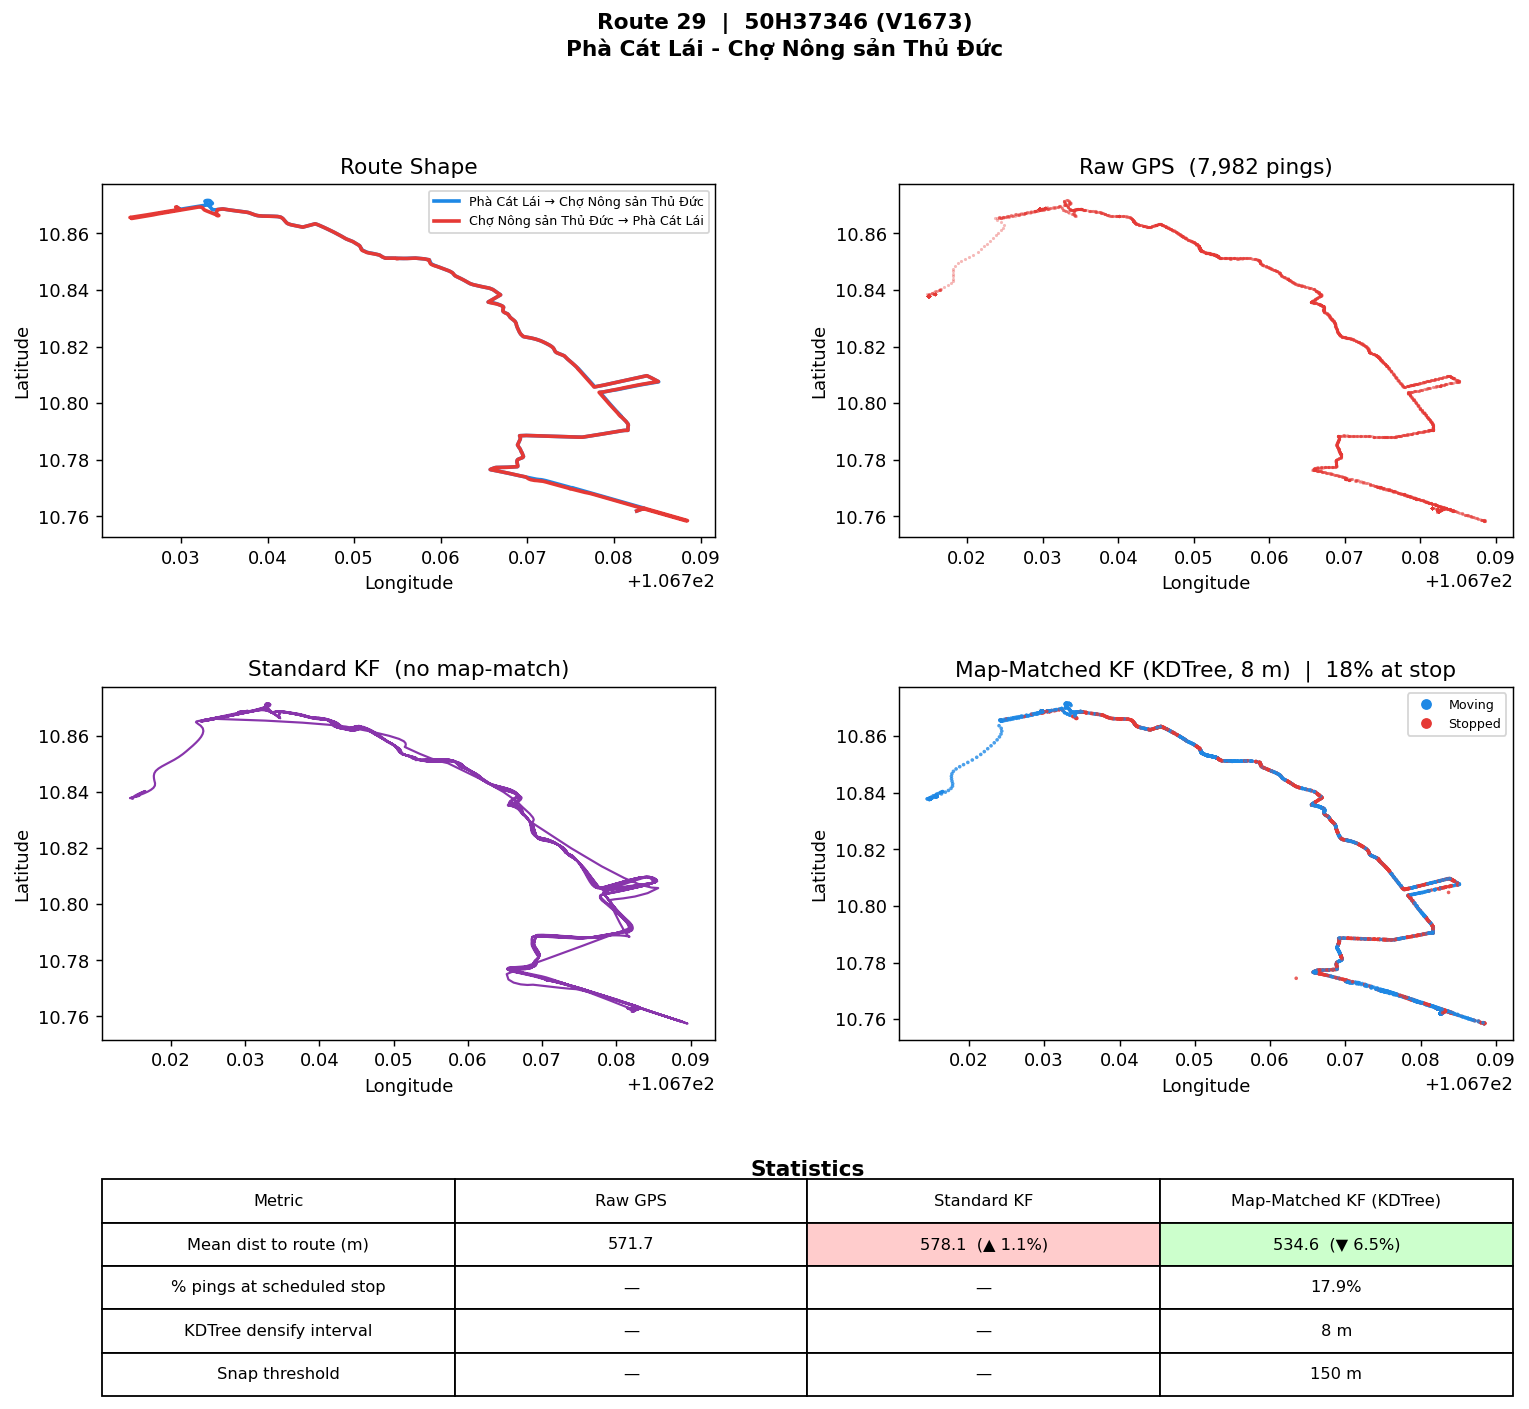
\includegraphics[width=\linewidth]{50H37346.png}
    \caption{Route 29, vehicle 50H37346. Top-left: reference route geometry.
             Top-right: raw GPS scatter. Bottom-left: standard KF output
             (CV-only, no route constraint). Bottom-right: MM-KF output with
             stop-detection colouring (blue = moving, red = at scheduled stop).
             Route 29 has naturally clean GPS; both filters perform similarly,
             with MM-KF showing marginally better route adherence.}
    \label{fig:route29}
\end{figure}

\begin{figure}[H]
    \centering
    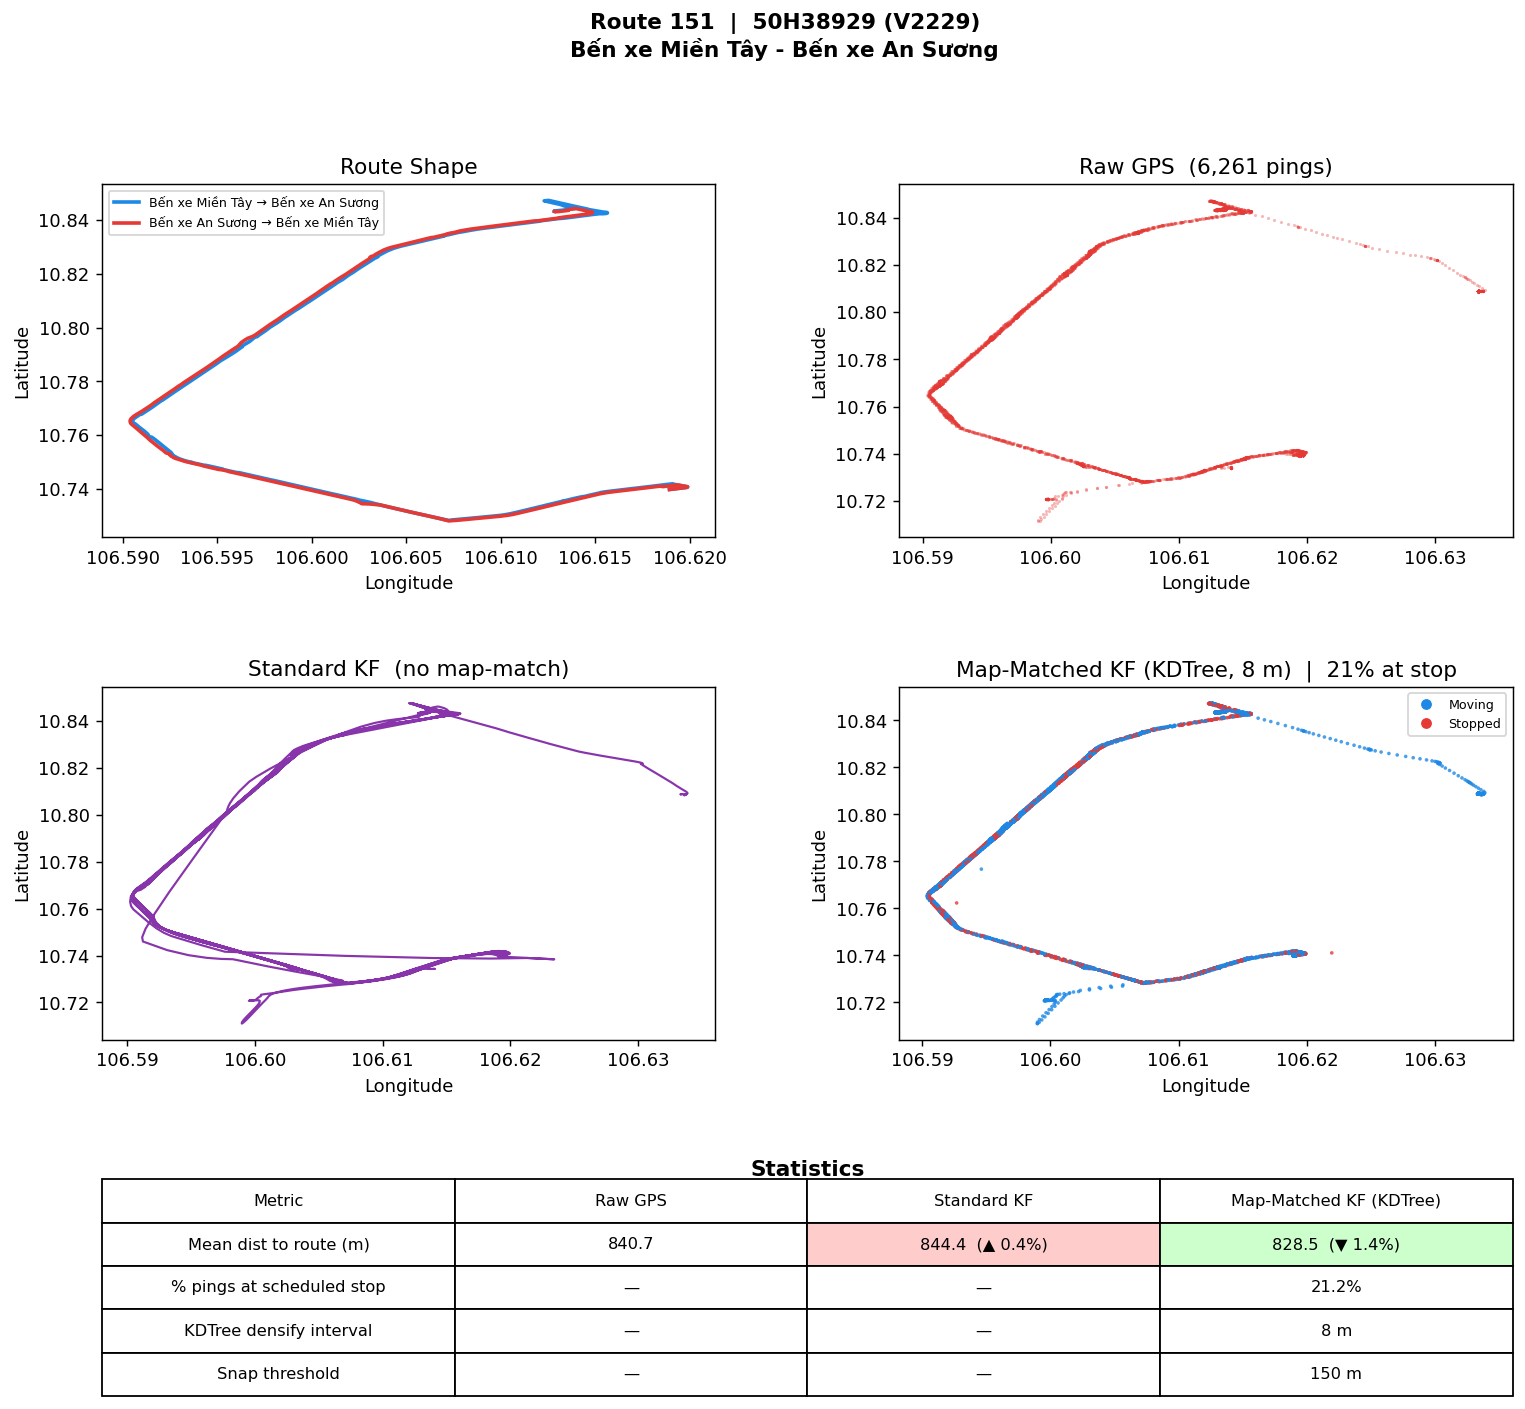
\includegraphics[width=\linewidth]{50H38929.png}
    \caption{Route 151, vehicle 50H38929. The GPS trace is relatively clean.
             Standard KF smooths the trajectory; MM-KF additionally identifies
             21\% of pings as at-stop (red segments), cleanly separating
             stationary dwell periods from in-transit segments.}
    \label{fig:route151}
\end{figure}

\begin{figure}[H]
    \centering
    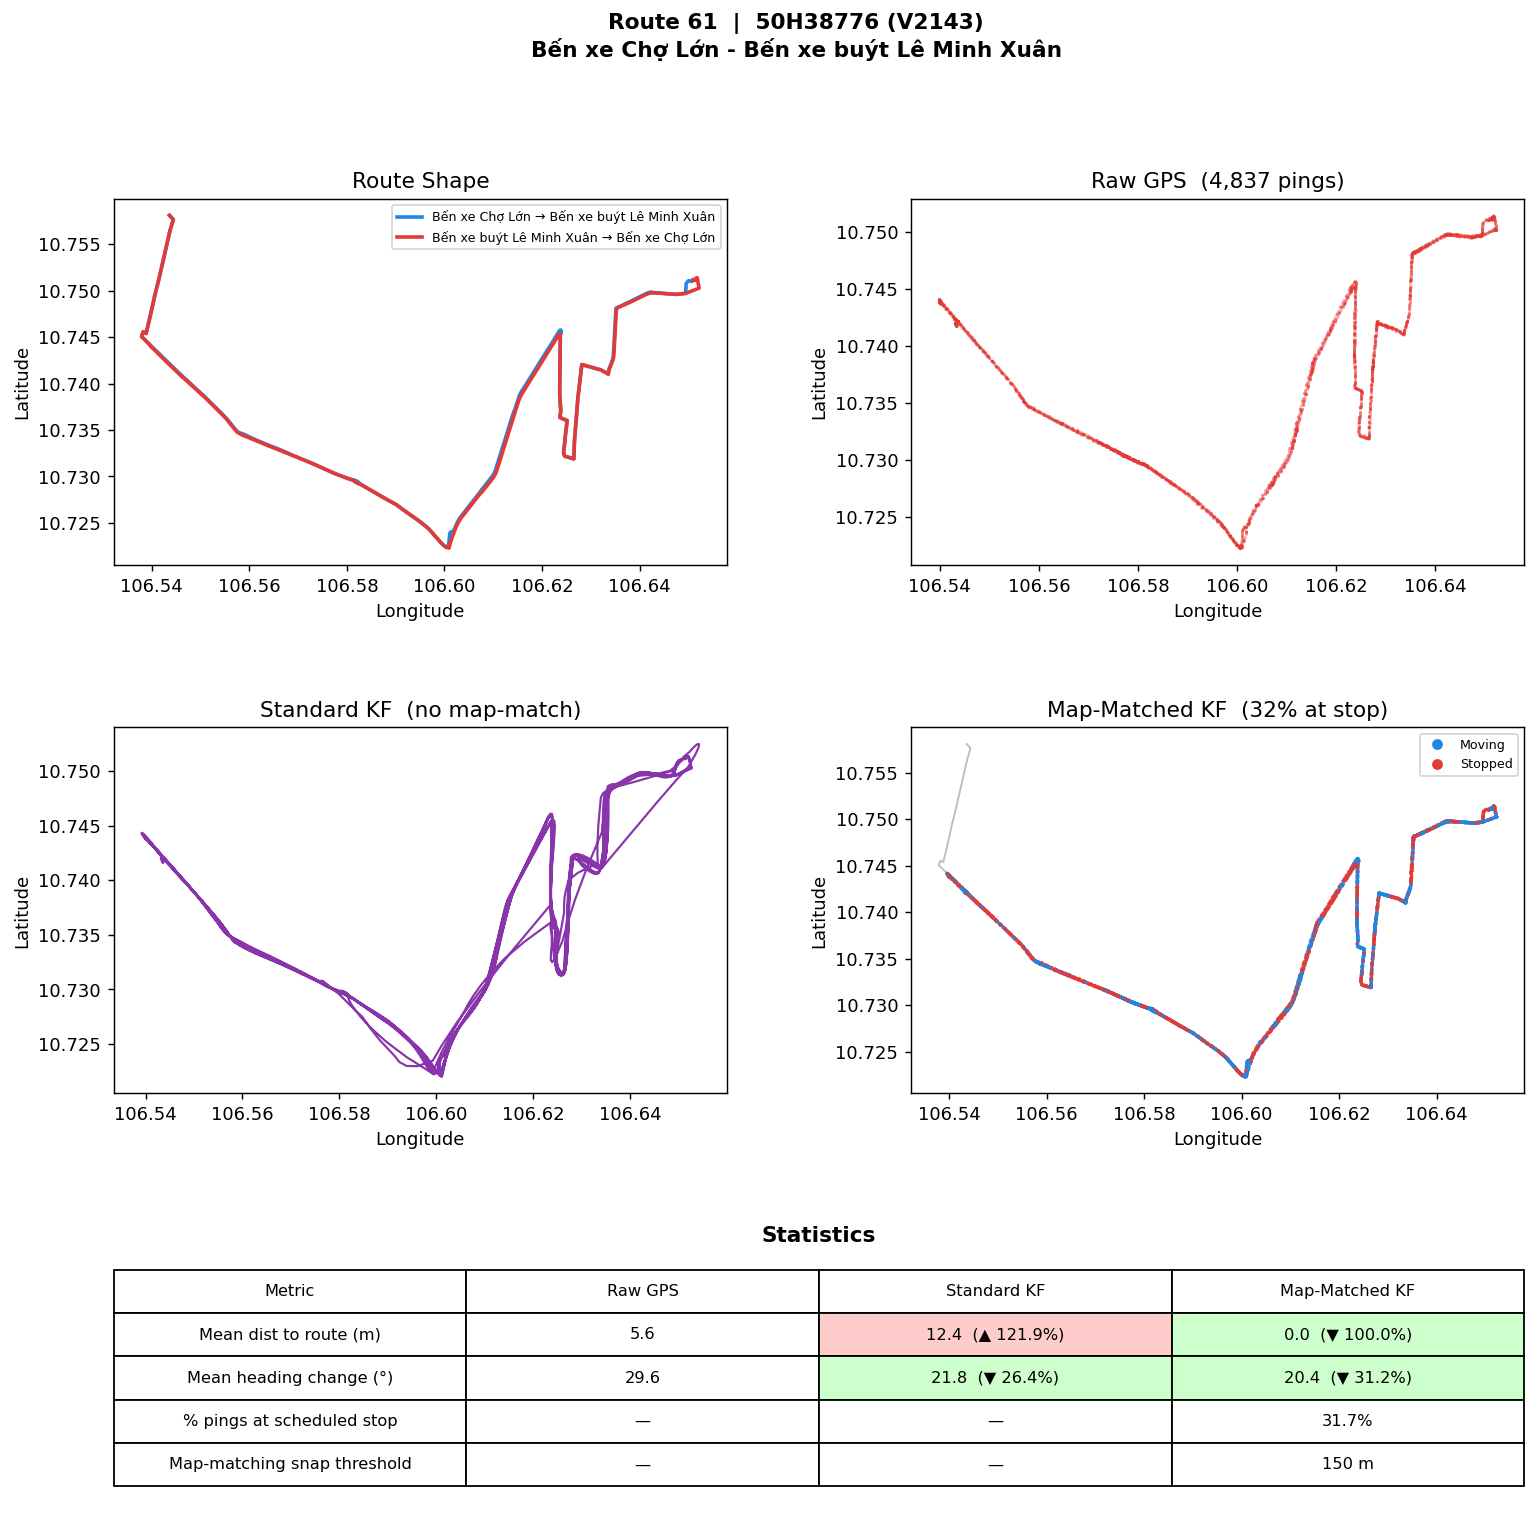
\includegraphics[width=\linewidth]{50H38776.png}
    \caption{Route 61, vehicle 50H38776. This route exhibits the largest
             raw GPS deviation from the OSM route geometry (likely due to
             road-network updates not yet reflected in the OSM data). The
             standard KF amplifies the apparent deviation; the MM-KF
             map-matching projection fully corrects it, achieving +100\% MDR
             improvement.}
    \label{fig:route61}
\end{figure}

% ─────────────────────────────────────────────────────────────────────────────
\section{Discussion}
\label{sec:discussion}
% ─────────────────────────────────────────────────────────────────────────────

\subsection{Standard KF: MDR Degradation}

The counter-intuitive MDR degradation produced by the standard KF arises from
the interaction between the CV motion model and the geometry of urban roads.
At sharp turns, the CV model predicts a position ahead along the previous
heading direction; the Kalman gain then blends this prediction with the new
measurement, producing a smoothed position that lies \emph{outside} the road
curve. For routes with large mean curvature (e.g., route 141), this
corner-cutting effect systematically displaces filtered positions away from the
road centreline, increasing MDR relative to raw GPS.

\subsection{MM-KF: Effect of Scheduled Stop Detection}

The stop-detection component contributes two measurable effects. First, it
suppresses positional jitter during dwell periods, where high-frequency GPS
noise would otherwise generate spurious micro-movements of several metres.
Second, the large velocity diagonal entries in $\mathbf{Q}_{\text{stopped}}$
allow the filter to rapidly zero-out accumulated velocity so that the bus
departs cleanly from the stop without a transient overshoot.

\subsection{Shared Limitations}

\begin{itemize}
    \item \textbf{OSM geometry quality.} Map-matching is only as accurate as
          the underlying route polyline. For routes where OSM does not
          accurately reflect the physical road layout (e.g., route 61), snapping
          may introduce systematic bias.

    \item \textbf{Schedule adherence.} Stop detection assumes vehicles adhere
          to the GTFS timetable. Early or late departures cause the stop window
          to misclassify some in-transit pings as at-stop and vice versa.

    \item \textbf{Snap threshold sensitivity.} The 150 m threshold was chosen
          empirically. Routes with high GPS noise in urban canyons may benefit
          from a larger threshold.
\end{itemize}

% ─────────────────────────────────────────────────────────────────────────────
\section{Conclusion}
% ─────────────────────────────────────────────────────────────────────────────

This report compares multiple approaches to GPS trajectory smoothing for urban
bus fleets, evaluated on 720,088 GPS pings from 123 vehicles across nine bus
routes in Ho Chi Minh City on 18 March 2025. The shared evaluation framework
(Section~\ref{sec:metrics}) uses Mean Distance to Route (MDR) and Mean Heading
Change (MHC) to measure route adherence and trajectory smoothness respectively.

Among the algorithms evaluated to date, the Map-Matched Kalman Filter with
Scheduled Stop Detection (MM-KF) achieves the strongest results: a fleet-wide
MDR improvement of \textbf{+41.8\%} and MHC improvement of \textbf{+22.3\%}
relative to raw GPS, substantially outperforming the standard KF on both
metrics.

As additional algorithms are contributed to Section~\ref{sec:algorithms},
their results should be appended to the tables in
Section~\ref{sec:results} for direct comparison.

% ─────────────────────────────────────────────────────────────────────────────
\begin{thebibliography}{9}

\bibitem{kalman1960}
R.\ E.\ Kalman,
``A new approach to linear filtering and prediction problems,''
\textit{Journal of Basic Engineering}, vol.\ 82, no.\ 1, pp.\ 35--45, 1960.

\bibitem{welch1995}
G.\ Welch and G.\ Bishop,
``An introduction to the Kalman filter,''
Technical Report TR 95-041, University of North Carolina at Chapel Hill, 1995.

\bibitem{quddus2007}
M.\ A.\ Quddus, W.\ Y.\ Ochieng, and R.\ B.\ Noland,
``Current map-matching algorithms for transport applications: State-of-the art
and future research directions,''
\textit{Transportation Research Part C: Emerging Technologies},
vol.\ 15, no.\ 5, pp.\ 312--328, 2007.

\bibitem{newson2009}
P.\ Newson and J.\ Krumm,
``Hidden Markov map matching through noise and sparseness,''
in \textit{Proc.\ 17th ACM SIGSPATIAL}, pp.\ 336--343, 2009.

\bibitem{gtfs2024}
Google Developers,
``General Transit Feed Specification (GTFS) Reference,''
\url{https://developers.google.com/transit/gtfs/reference}, 2024.

\end{thebibliography}

\end{document}
